\tikzset{every picture/.style={line width=0.75pt}} %set default line width to 0.75pt        

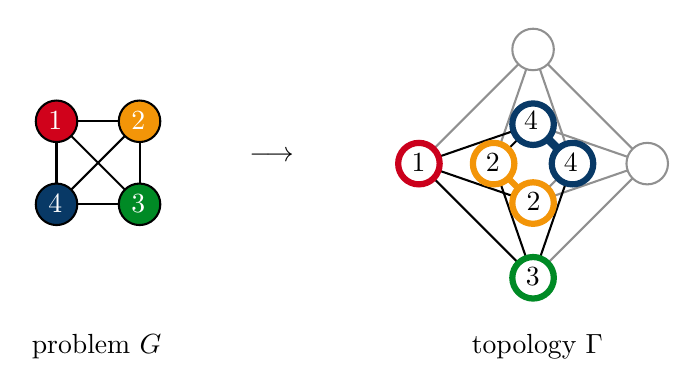
\begin{tikzpicture}[x=0.75pt,y=0.75pt,yscale=-1,xscale=1]

\draw [color={rgb, 255:red, 144; green, 144; blue, 144 }  ,draw opacity=1 ]   (255,12.4) -- (310,67.4) ;
\draw [color={rgb, 255:red, 144; green, 144; blue, 144 }  ,draw opacity=1 ]   (310,67.4) -- (255,122.4) ;
\draw [color={rgb, 255:red, 144; green, 144; blue, 144 }  ,draw opacity=1 ]   (255,12.4) -- (200,67.4) ;
\draw    (200,67.4) -- (255,122.4) ;
\draw [color={rgb, 255:red, 243; green, 149; blue, 8 }  ,draw opacity=1 ][line width=2.25]    (236,67.4) -- (255,86.4) ;
\draw [color={rgb, 255:red, 8; green, 57; blue, 102 }  ,draw opacity=1 ][line width=3]    (255,48.4) -- (274,67.4) ;
\draw    (236,67.4) -- (255,48.4) ;
\draw [color={rgb, 255:red, 144; green, 144; blue, 144 }  ,draw opacity=1 ]   (255,86.4) -- (274,67.4) ;
\draw [color={rgb, 255:red, 0; green, 0; blue, 0 }  ,draw opacity=1 ]   (200,67.4) -- (255,86.4) ;
\draw [color={rgb, 255:red, 144; green, 144; blue, 144 }  ,draw opacity=1 ]   (310,67.4) -- (255,48.4) ;
\draw [color={rgb, 255:red, 144; green, 144; blue, 144 }  ,draw opacity=1 ]   (310,67.4) -- (255,86.4) ;
\draw  [color={rgb, 255:red, 144; green, 144; blue, 144 }  ,draw opacity=1 ][fill={rgb, 255:red, 255; green, 255; blue, 255 }  ,fill opacity=1 ] (310,57.4) .. controls (315.52,57.4) and (320,61.88) .. (320,67.4) .. controls (320,72.92) and (315.52,77.4) .. (310,77.4) .. controls (304.48,77.4) and (300,72.92) .. (300,67.4) .. controls (300,61.88) and (304.48,57.4) .. (310,57.4) -- cycle ;
\draw    (25.4,47) -- (65.4,47) ;
\draw    (25.4,87) -- (65.4,87) ;
\draw    (25.4,47) -- (25.4,87) ;
\draw    (65.4,47) -- (65.4,87) ;
\draw    (25.4,47) -- (65.4,87) ;
\draw    (65.4,47) -- (25.4,87) ;
\draw  [fill={rgb, 255:red, 208; green, 2; blue, 27 }  ,fill opacity=1 ] (15.4,47) .. controls (15.4,41.48) and (19.88,37) .. (25.4,37) .. controls (30.92,37) and (35.4,41.48) .. (35.4,47) .. controls (35.4,52.52) and (30.92,57) .. (25.4,57) .. controls (19.88,57) and (15.4,52.52) .. (15.4,47) -- cycle ;
\draw  [fill={rgb, 255:red, 243; green, 149; blue, 8 }  ,fill opacity=1 ] (55.4,47) .. controls (55.4,41.48) and (59.88,37) .. (65.4,37) .. controls (70.92,37) and (75.4,41.48) .. (75.4,47) .. controls (75.4,52.52) and (70.92,57) .. (65.4,57) .. controls (59.88,57) and (55.4,52.52) .. (55.4,47) -- cycle ;
\draw  [fill={rgb, 255:red, 8; green, 57; blue, 102 }  ,fill opacity=1 ] (15.4,87) .. controls (15.4,81.48) and (19.88,77) .. (25.4,77) .. controls (30.92,77) and (35.4,81.48) .. (35.4,87) .. controls (35.4,92.52) and (30.92,97) .. (25.4,97) .. controls (19.88,97) and (15.4,92.52) .. (15.4,87) -- cycle ;
\draw  [fill={rgb, 255:red, 0; green, 138; blue, 37 }  ,fill opacity=1 ] (55.4,87) .. controls (55.4,81.48) and (59.88,77) .. (65.4,77) .. controls (70.92,77) and (75.4,81.48) .. (75.4,87) .. controls (75.4,92.52) and (70.92,97) .. (65.4,97) .. controls (59.88,97) and (55.4,92.52) .. (55.4,87) -- cycle ;
\draw [color={rgb, 255:red, 144; green, 144; blue, 144 }  ,draw opacity=1 ][line width=0.75]    (255,12.4) -- (236,67.4) ;
\draw    (274,67.4) -- (255,122.4) ;
\draw [color={rgb, 255:red, 144; green, 144; blue, 144 }  ,draw opacity=1 ]   (255,12.4) -- (274,67.4) ;
\draw  [color={rgb, 255:red, 8; green, 57; blue, 102 }  ,draw opacity=1 ][fill={rgb, 255:red, 255; green, 255; blue, 255 }  ,fill opacity=1 ][line width=2.25]  (274,57.4) .. controls (279.52,57.4) and (284,61.88) .. (284,67.4) .. controls (284,72.92) and (279.52,77.4) .. (274,77.4) .. controls (268.48,77.4) and (264,72.92) .. (264,67.4) .. controls (264,61.88) and (268.48,57.4) .. (274,57.4) -- cycle ;
\draw  [color={rgb, 255:red, 144; green, 144; blue, 144 }  ,draw opacity=1 ][fill={rgb, 255:red, 255; green, 255; blue, 255 }  ,fill opacity=1 ][line width=0.75]  (245,12.4) .. controls (245,6.88) and (249.48,2.4) .. (255,2.4) .. controls (260.52,2.4) and (265,6.88) .. (265,12.4) .. controls (265,17.92) and (260.52,22.4) .. (255,22.4) .. controls (249.48,22.4) and (245,17.92) .. (245,12.4) -- cycle ;
\draw    (200,67.4) -- (255,48.4) ;
\draw    (236,67.4) -- (255,122.4) ;
\draw  [color={rgb, 255:red, 243; green, 149; blue, 8 }  ,draw opacity=1 ][fill={rgb, 255:red, 255; green, 255; blue, 255 }  ,fill opacity=1 ][line width=2.25]  (236,57.4) .. controls (241.52,57.4) and (246,61.88) .. (246,67.4) .. controls (246,72.92) and (241.52,77.4) .. (236,77.4) .. controls (230.48,77.4) and (226,72.92) .. (226,67.4) .. controls (226,61.88) and (230.48,57.4) .. (236,57.4) -- cycle ;
\draw  [color={rgb, 255:red, 243; green, 149; blue, 8 }  ,draw opacity=1 ][fill={rgb, 255:red, 255; green, 255; blue, 255 }  ,fill opacity=1 ][line width=2.25]  (245,86.4) .. controls (245,80.88) and (249.48,76.4) .. (255,76.4) .. controls (260.52,76.4) and (265,80.88) .. (265,86.4) .. controls (265,91.92) and (260.52,96.4) .. (255,96.4) .. controls (249.48,96.4) and (245,91.92) .. (245,86.4) -- cycle ;
\draw  [color={rgb, 255:red, 8; green, 57; blue, 102 }  ,draw opacity=1 ][fill={rgb, 255:red, 255; green, 255; blue, 255 }  ,fill opacity=1 ][line width=2.25]  (245,48.4) .. controls (245,42.88) and (249.48,38.4) .. (255,38.4) .. controls (260.52,38.4) and (265,42.88) .. (265,48.4) .. controls (265,53.92) and (260.52,58.4) .. (255,58.4) .. controls (249.48,58.4) and (245,53.92) .. (245,48.4) -- cycle ;
\draw  [color={rgb, 255:red, 203; green, 0; blue, 28 }  ,draw opacity=1 ][fill={rgb, 255:red, 255; green, 255; blue, 255 }  ,fill opacity=1 ][line width=2.25]  (200,57.4) .. controls (205.52,57.4) and (210,61.88) .. (210,67.4) .. controls (210,72.92) and (205.52,77.4) .. (200,77.4) .. controls (194.48,77.4) and (190,72.92) .. (190,67.4) .. controls (190,61.88) and (194.48,57.4) .. (200,57.4) -- cycle ;
\draw  [color={rgb, 255:red, 0; green, 138; blue, 37 }  ,draw opacity=1 ][fill={rgb, 255:red, 255; green, 255; blue, 255 }  ,fill opacity=1 ][line width=2.25]  (245,122.4) .. controls (245,116.88) and (249.48,112.4) .. (255,112.4) .. controls (260.52,112.4) and (265,116.88) .. (265,122.4) .. controls (265,127.92) and (260.52,132.4) .. (255,132.4) .. controls (249.48,132.4) and (245,127.92) .. (245,122.4) -- cycle ;

\draw (20,41) node [anchor=north west][inner sep=0.75pt]  [color={rgb, 255:red, 255; green, 255; blue, 255 }  ,opacity=1 ] [align=left] {1};
\draw (60,41) node [anchor=north west][inner sep=0.75pt]  [color={rgb, 255:red, 255; green, 255; blue, 255 }  ,opacity=1 ] [align=left] {2};
\draw (60,81) node [anchor=north west][inner sep=0.75pt]  [color={rgb, 255:red, 255; green, 255; blue, 255 }  ,opacity=1 ] [align=left] {3};
\draw (20,81) node [anchor=north west][inner sep=0.75pt]  [color={rgb, 255:red, 255; green, 255; blue, 255 }  ,opacity=1 ] [align=left] {4};
\draw (250,116) node [anchor=north west][inner sep=0.75pt]   [align=left] {3};
\draw (195,61) node [anchor=north west][inner sep=0.75pt]   [align=left] {1};
\draw (250.4,80) node [anchor=north west][inner sep=0.75pt]   [align=left] {2};
\draw (230.8,61) node [anchor=north west][inner sep=0.75pt]   [align=left] {2};
\draw (249.2,41) node [anchor=north west][inner sep=0.75pt]   [align=left] {4};
\draw (268.4,61) node [anchor=north west][inner sep=0.75pt]   [align=left] {4};
\draw (116.8,60) node [anchor=north west][inner sep=0.75pt]    {$\longrightarrow $};
\draw (224,148) node [anchor=north west][inner sep=0.75pt]{topology $\Gamma$};
\draw (12,148) node [anchor=north west][inner sep=0.75pt]{problem $G$};

\end{tikzpicture}